\documentclass[8pt]{beamer} % dvipsnames gives more built-in colors
\usepackage{graphicx}

\usetheme{Madrid}
\useoutertheme{miniframes} % Alternatively: miniframes, infolines, split
\useinnertheme{circles}

\definecolor{UBCblue}{rgb}{0.04706, 0.13725, 0.26667} % UBC Blue (primary)

\usecolortheme[named=UBCblue]{structure}
%\usecolortheme[named=Mahogany]{structure} % Sample dvipsnames color



\title{Paper Review - Auto-FuzzyJoin: Auto-Program Fuzzy Similarity Joins Without Labelled Examples}
\subtitle{Peng Li, Xiang Cheng, Xu Chu, Yeye He, Surajit Chaudhuri}
\date{\today}
\author{Carmel Gafa}


\begin{document}

\setbeamercolor{definition}{bg=red!10, fg=black}
\setbeamercolor{code}{bg=gray!15!white, fg=black}
\setbeamercolor{example}{bg=yellow!10, fg=black}


\begin{frame}[plain]
    \maketitle
\end{frame}

\small
\begin{frame}{Fuzzy-join (or similarity join)}
	\begin{figure}
		\centering
		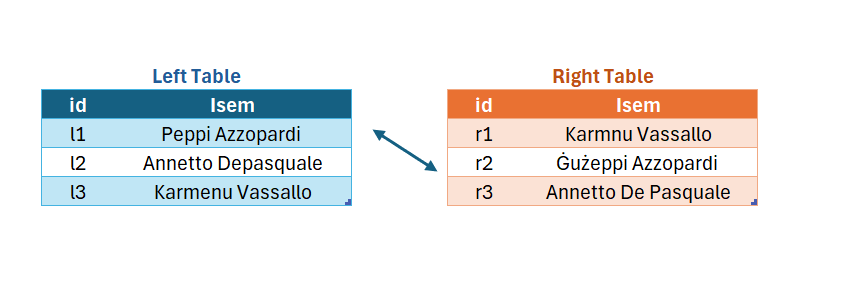
\includegraphics[width=0.7\linewidth]{FuzzyJoin}
	\end{figure}

	\begin{figure}
		\centering
		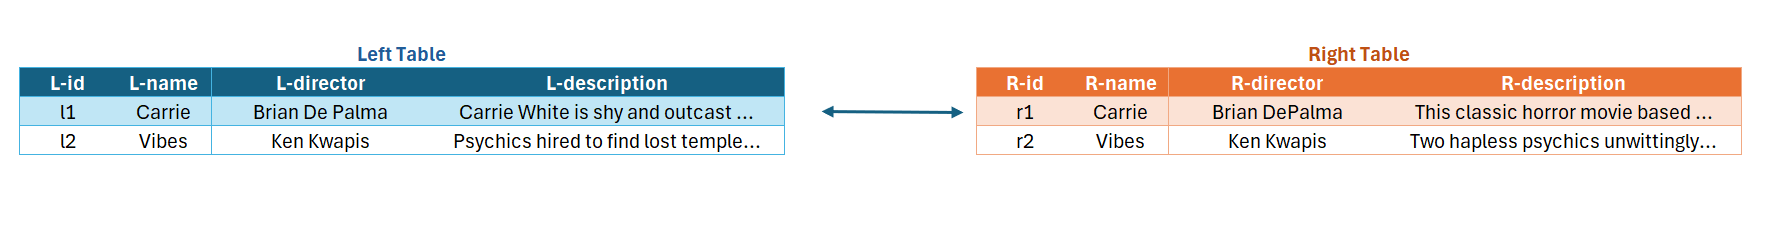
\includegraphics[width=1\linewidth]{img/FuzzyJoin_2}
	\end{figure}

	\begin{itemize}
		\item Fuzzy join takes two tables as inputs and identifies record pairs that refer to the same entity.
		\item As an example, l1 and r2 refer to the same person.
		\item The concept can be extended to records with multiple fields or attributes.
	\end{itemize}
\end{frame}


\begin{frame}{Fuzzy-join configuration }
	 \begin{tabular}{ccc}  
		\begin{tabular}{c}
			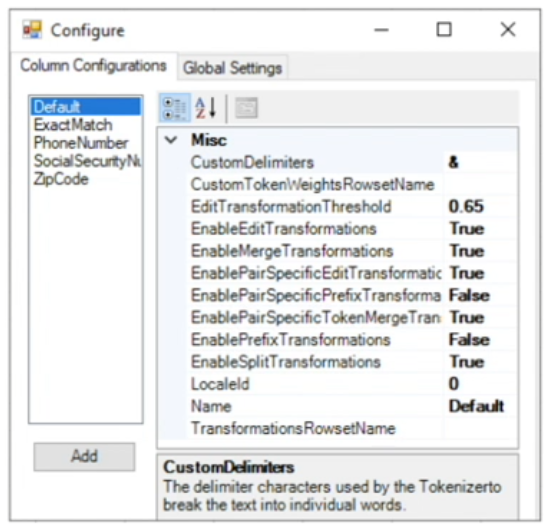
\includegraphics[width=0.2\linewidth]{img/FuzzyJoin_config_1.png}
		\end{tabular}
		& \begin{tabular}{l}
			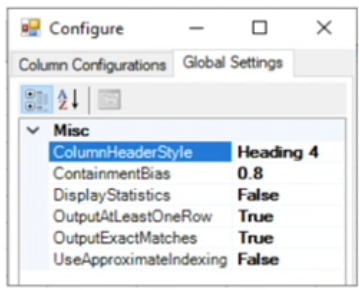
\includegraphics[width=0.2\linewidth]{img/FuzzyJoin_config_2.png}
		\end{tabular}	
		& \begin{tabular}{l}
		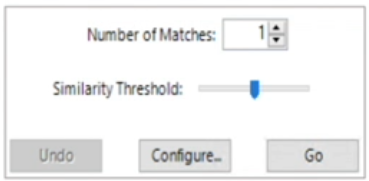
\includegraphics[width=0.2\linewidth]{img/FuzzyJoin_config_3.png}
		\end{tabular}  \\
	\end{tabular}
	
	\begin{itemize}
		\item Fuzzy-join has been integrated into many commercial applications
		\item These systems are often difficult to use due to the large number of configuration parameters.
		\item The extension in Microsoft Excel has 19 options that span across 3 dialog boxes.
		\begin{itemize}
			\item 11 are binary, thus resulting in 2048 possible configuration scenarios.
			\item 8 continuous, such as thresholds and biases.
		\end{itemize}
		\item In order to execute quality Fuzzy-joins, these configurations require careful user setup to achieve high-quality results.
	\end{itemize}
\end{frame}



%-----------------------------------------------------------------------------------------------------------------------------

\begin{frame}{Theoretical foundation: fuzzy join mapping}
	Given a \textbf{reference table} $L$ and a table $R$ containing records that may be \textbf{imprecise} or noisy, a \textbf{fuzzy join mapping} $J$ establishes approximate matches between them.
	
	\begin{itemize}
	\item $J$ connects elements of $R$ to similar elements in $L$ based on a chosen \textbf{similarity measure} (e.g., Levenshtein distance, cosine similarity, Jaccard similarity).
	\item Each record $r \in R$ is mapped to at most one record $l \in L$, or \textbf{no match at all} (denoted by $\perp$).
	\item The join is \textbf{many-to-one} because multiple records in $R$ can be associated with the \textbf{same} record in $L$, but each $r \in R$ has only \textbf{one} possible match.
	\end{itemize}
	
	Formally:
	\begin{beamercolorbox}[rounded=true, shadow=true, leftskip=1em, rightskip=1em]{definition}
		$$
		J: R \rightarrow L \cup \bot
		$$
	\end{beamercolorbox}
\end{frame}


\begin{frame}{Theoretical foundation: fuzzy join configuration space}
	A \textbf{fuzzy join} $f$ compares two strings, $r$ and $l$, by computing a distance score that reflects their similarity. The computation of this score is governed by a variety of parameters, forming a \textbf{parameter space}. 
	
	\vspace{1em}

	\begin{beamercolorbox}[rounded=true, shadow=true, leftskip=1em, rightskip=1em]{definition}
		Each unique combination of these parameters defines a specific \textbf{join function} $f \in \mathcal{F}$, where $\mathcal{F}$ is the space of all possible join functions.
	\end{beamercolorbox}

	\vspace{1em}
		
	\begin{figure}
		\centering
				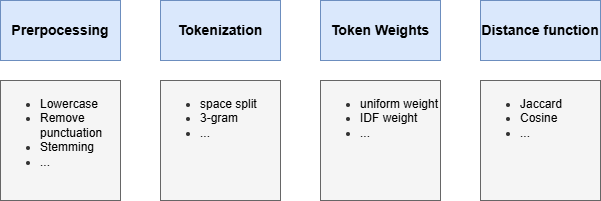
\includegraphics[width=0.7\linewidth]{img/join_configuration.png}
	\end{figure}
\end{frame}



\begin{frame}{Example: fuzzy join distance score computation}
	
	\tiny
	\begin{beamercolorbox}[rounded=true, shadow=true, leftskip=1em, rightskip=1em]{example}
		\textbf{Join Function:} $f = (L, SP, EW, JD)$
		\begin{itemize}
			\item \textbf{L}: Lower-casing (Preprocessing)
			\item \textbf{SP}: Space Tokenization
			\item \textbf{EW}: Equal Weights
			\item \textbf{JD}: Jaccard Distance
		\end{itemize}
		
		\vspace{1em}
		\textbf{Inputs:}
		\begin{itemize}
			\item $l = \texttt{"2012 tigers lsu baseball team"}$
			\item $r = \texttt{"2012 lsu baseball team"}$
		\end{itemize}
		
		\vspace{1em}
		\textbf{Tokenization (SP):}
		\begin{itemize}
			\item $l \rightarrow \{2012, tigers, lsu, baseball, team\}$
			\item $r \rightarrow \{2012, lsu, baseball, team\}$
		\end{itemize}
		
		\vspace{1em}
		\textbf{Jaccard Distance:}
		\begin{itemize}
			\item $A \cap B = \{2012, lsu, baseball, team\} \rightarrow |A \cap B| = 4$
			\item $A \cup B = \{2012, tigers, lsu, baseball, team\} \rightarrow |A \cup B| = 5$
			\item $\text{Jaccard Similarity} = \frac{4}{5} = 0.8$
			\item $\text{Jaccard Distance} = 1 - 0.8 = 0.2$
		\end{itemize}
		
		\vspace{1em}
		\textbf{Result:} $f(l, r) = 0.2$
	\end{beamercolorbox}
\end{frame}


\begin{frame}{Theoretical foundation: threshold and join configuration}
		
	\begin{itemize}
		\item Once the distance $f(l, r)$ is computed:
		\begin{itemize}
			\item It is compared to a threshold \textbf{compared to a threshold} $\theta$  to decide whether to join the string pair $l$ and $r$.
			\begin{itemize}
				\item lower $\theta$ gives stricter matches
			\end{itemize}
			\item If $f(l, r) \leq \theta$ , the pair is considered \textbf{a match}.
		\end{itemize}
		\item 	Together, the function $f$ and the threshold $\theta$ define what the authors call a \textbf{join configuration}:$$
		C = \langle f, \theta \rangle
		$$
		\item This configuration encapsulates both:
		\begin{itemize}
			\item How distance is computed.
			\item When two strings are considered similar enough to be joined.
		\end{itemize}
	\end{itemize}	
	
	\vspace{1em}
	
	\begin{beamercolorbox}[rounded=true, shadow=true, leftskip=1em, rightskip=1em]{definition}
		A join configuration $C$ is a 2-tuple $C = \langle f, \theta \rangle$, where $f \in \mathcal{F}$ is a join function, and $\theta$ is a threshold.\\
		We use $\mathcal{S} = \{ \langle f, \theta \rangle \mid f \in \mathcal{F}, \theta \in \mathbb{R} \}$ to denote the space of join configurations.
	\end{beamercolorbox}

\end{frame}


\begin{frame}{Theoretical foundation: fuzzy join mapping}
	Given two tables $L$  and $R$ , a join configuration $C \in \mathcal{S}$ induces a \textbf{fuzzy join mapping} $J_C$ , defined as:
	
	\vspace{1em}
	
	\begin{beamercolorbox}[rounded=true, shadow=true, leftskip=1em, rightskip=1em]{definition}
	$$
		J_C(r) = \underset{l \in L,\ f(l, r) \leq \theta}{\arg\min} f(l, r),\ \forall r \in R
	$$
	\end{beamercolorbox}
	
	\vspace{1em}
	
	That is
	\begin{itemize}
		\item For each record $r \in R$, find $l \in L$ that minimizes the distance $f(l, r)$, \textbf{only if} that distance is less than or equal to the threshold $\theta$.
		\item If no such $l \in L$ exists such that $f(l, r) \leq \theta$, then $J_C(r)$ is maps to $\perp$ — i.e., no match for that record.
	\end{itemize}

\end{frame}


\begin{frame}{Theoretical foundation: the problem with single join configurations}
	
	\begin{columns}
		% Left column: explanation
		\begin{column}{0.52\textwidth}
			Real-world data can exhibit \textbf{multiple types of variations simultaneously}, such as:
			\begin{itemize}
				\item \textbf{Typos}
				\item \textbf{Missing tokens}
				\item \textbf{Extraneous information}
			\end{itemize}
			
			As a result, relying on a \textbf{single join configuration} often fails to capture all valid matches, particularly when high \textbf{recall} is required.
			
			\vspace{0.5em}
			To handle this diversity, the algorithm uses a \textbf{set of join configurations}:
			$$
			U = \{C_1, C_2, \dots, C_K\}
			$$
			
			Instead of relying on a single configuration, the system computes join results from each one.
			
			This approach allows the system to:
			\begin{itemize}
				\item Accommodate diverse types of variations.
				\item Improve overall recall by \textbf{combining multiple perspectives} on similarity (different parametrizations that are sensitive to different types of noise).
			\end{itemize}
		\end{column}
		
		
		\begin{column}{0.45\textwidth}
			
			\begin{beamercolorbox}[rounded=true, shadow=true, leftskip=1em, rightskip=1em]{example}
			
				\centering
				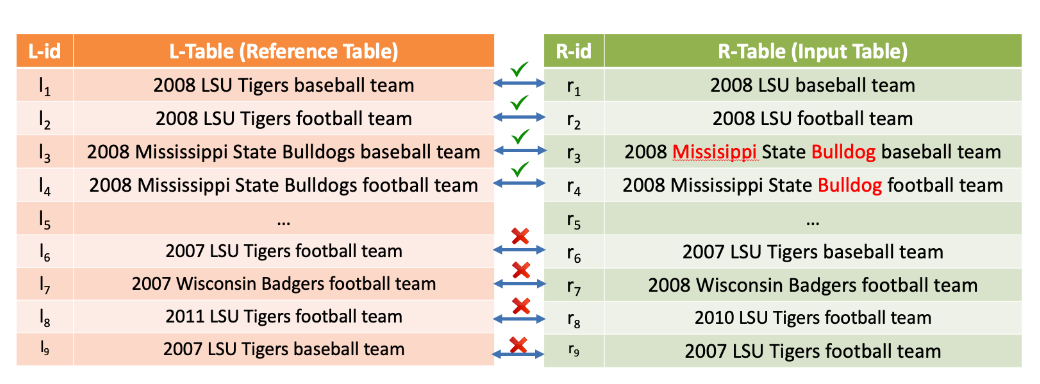
\includegraphics[width=\linewidth]{img/Pasted image 20250331152324.png}
				
				
				\vspace{0.5em}
				\small
				\begin{itemize}
					\item A \textbf{Jaccard distance} with threshold $0.2$ works well for pairs like $(l_1, r_1)$, which differ by only one or two tokens.
					\item However, for pairs like $(l_3, r_3)$ with \textbf{spelling variations}, Jaccard similarity is not enough:
					\begin{itemize}
						\item Jaccard distance $\approx 0.5 \rightarrow$ too high to match under the 0.2 threshold
						\item A more suitable metric is \textbf{Edit Distance}, which can better align such pairs.
					\end{itemize}
				\end{itemize}
			
		\end{beamercolorbox}
		
		\end{column}

	\end{columns}
	
\end{frame}



\begin{frame}{Theoretical foundation: fuzzy join via multiple configurations}
	
	\begin{itemize}
		\item To handle this diversity, the algorithm uses a \textbf{set of join configurations}:
		$$
		U = \{C_1, C_2, \dots, C_K\}
		$$
		\item Instead of relying on a single configuration, the system computes join results from each.
		\item This approach allows the system to:
		\begin{itemize}
			\item Accommodate diverse types of variations.
			\item Improve overall recall by \textbf{combining multiple perspectives} on similarity.
		\end{itemize}
	\end{itemize}
	
	\vspace{1em}

	\begin{beamercolorbox}[rounded=true, shadow=true, leftskip=1em, rightskip=1em]{definition}
		Given $L$ and $R$, a set of join configurations $U = \{C_1, C_2, \ldots, C_K\}$ induces a \textbf{fuzzy join mapping} $J_U$, defined as:
		$$
		J_U(r) = \bigcup_{C_i \in U} J_{C_i}(r),\ \forall r \in R
		$$
		This means that the overall result of the fuzzy join using configuration set $U$ is the \textbf{union} of results from all individual configurations $C_i \in U$.
	\end{beamercolorbox}
	
	\vspace{0.5em}
	
	Each configuration $C_i \in U$ is designed to capture a \textbf{specific type of string variation} (e.g., typos, missing tokens, extra tokens).
	
	Two records are considered \textbf{joined by the set} $U$ \textbf{if and only if} they are joined by \textbf{at least one} configuration $C_i \in U$.
	
	\begin{itemize}
		\item Each configuration contributes \textbf{high-quality joins} targeted at particular data challenges.
		\item The overall join is more \textbf{robust and comprehensive}.
	\end{itemize}
\end{frame}


\begin{frame}{Theoretical foundation: evaluating join quality; Precision}
	
	Given two tables $R$ and $L$, and a \textbf{space of join configurations} $\mathcal{S}$, the objective is to find a subset $U \subseteq \mathcal{S}$ that produces \textbf{good fuzzy join results}.
	
	Let:
	\begin{itemize}
		\item $J_U$ be the fuzzy join mapping induced by configuration set $U$
		\item $J_G$ be the \textbf{ground truth} join mapping — the ideal join result
	\end{itemize}
	
	\vspace{0.5em}
	
	\begin{beamercolorbox}[rounded=true, shadow=true, leftskip=1em, rightskip=1em]{definition}
		\textbf{Precision} measures how many of the predicted joins are correct:
		
		$$
		\text{precision}(U) =
		\frac{
			\underbrace{|\{ r \in R\ |\ J_U(r) \neq \emptyset,\ J_U(r) = J_G(r) \}|}_{\text{True Positives (TP)}}
		}{
			\underbrace{|\{ r \in R\ |\ J_U(r) \neq \emptyset \}|}_{\text{TP + FP (all predicted joins)}}
		}
		$$
	\end{beamercolorbox}
	
	\begin{itemize}
		\item \textbf{Numerator (TP)}: Records where a join was predicted and it matched the ground truth.
		\item \textbf{Denominator (TP + FP)}: All records where a join was predicted (correct or not).
		\item Only records with a prediction (i.e., $J_U(r) \neq \emptyset$) are evaluated in this precision formula.
	\end{itemize}
	
\end{frame}


\begin{frame}{Theoretical foundation: evaluating join quality; Recall}
	
	\begin{beamercolorbox}[rounded=true, shadow=true, leftskip=1em, rightskip=1em]{definition}
		\textbf{Recall} measures how many of the correct (ground truth) joins were successfully predicted:
		
		$$
		\text{recall}(U) =
		\underbrace{|\{ r \in R\ |\ J_U(r) \neq \emptyset,\ J_U(r) = J_G(r) \}|}_{\text{True Positives (TP)}}
		$$
	\end{beamercolorbox}
	
	\vspace{1em}
	
	\begin{itemize}
		\item This is the \textbf{absolute count of True Positives}, i.e., records for which:
		\begin{itemize}
			\item A join was predicted ($J_U(r) \neq \emptyset$), and
			\item It matches the ground truth ($J_U(r) = J_G(r)$)
		\end{itemize}
	\end{itemize}
	
	\vspace{0.5em}
	\textbf{False Negatives (FN)} — cases where a correct join was missed — are defined as:
	$$
	\text{FN} = |\{ r \in R\ |\ J_G(r) \neq \emptyset,\ J_U(r) = \emptyset \}|
	$$
	
	\textit{Note:} The denominator $TP + FN$ is constant across all $U$ for a fixed dataset, so it is omitted in comparisons.
	
\end{frame}



\begin{frame}{Theoretical foundation: Estimating precision without labels}
	

	\textbf{Traditional precision metrics require a labeled ground truth to evaluate the quality of predicted joins.}
	
	\vspace{1em}
	
	\textbf{Auto-FuzzyJoin introduces an unsupervised method to estimate join precision, without labeled data.}
	
	\vspace{1em}
	\begin{itemize}
		\item Uses a local geometric heuristic: the number of $L$ records within a $2d$-ball around a matched reference point $l$
		\item Fewer neighbors imply higher confidence in the match (i.e., higher estimated precision)
		\item This estimation is:
		\begin{itemize}
			\item \textbf{Data-driven}: only needs $L$ and $R$
			\item \textbf{Model-independent}: works with any join function $f$
			\item \textbf{Efficient}: avoids costly labeling efforts
		\end{itemize}
	\end{itemize}
	
	\vspace{0.5em}
	\textit{This idea enables precision-aware optimization without needing ground truth labels.}
	
\end{frame}


\begin{frame}{Theoretical foundation: estimating Precision/Recall for a single join configuration}
	
	Given:
	\begin{itemize}
		\item A \textbf{single join configuration} $C = \langle f, \theta \rangle$
		\item Two tables:
		\begin{itemize}
			\item $L$: reference table
			\item $R$: query table
		\end{itemize}
	\end{itemize}
	
	\vspace{0.5em}
	\textbf{Assumption: Complete Reference Table $L$}
	\begin{itemize}
		\item $L$ is assumed to contain \textbf{all possible true matches} for records in $R$.
		\item Ensures that for each $r \in R$, there exists a correct match $l \in L$.
		\item Simplifies analysis by reducing the chance of missing true positives due to an incomplete reference.
	\end{itemize}
	
	\vspace{0.5em}
	\textbf{Geometric View of the Distance Function $f$}
	\begin{itemize}
		\item Join function $f$ embeds records into a \textbf{metric space}.
		\item Records are conceptually modelled as points on a \textbf{unit grid}.
		\item Each $l \in L$ is surrounded by \textbf{close variants} (differing by a token, character, etc.).
		\item The distance between each $l$ and the surrounding $r$'s is exploited by $\theta$ to compute join pairs.
	\end{itemize}
	
	\vspace{0.5em}
	\setbeamercolor{block title}{bg=green!10, fg=black}
	\setbeamercolor{block body}{bg=green!5, fg=black}
	\begin{block}{Analogy: Stars and Planets}
		\begin{itemize}
			\item Reference records $l \in L$ are like \textbf{stars} on a grid.
			\item Query records $r \in R$ are like \textbf{planets} that orbit these stars.
			\item Identifying the best join $J_C(r)$ is like determining \textbf{which star a planet orbits}.
		\end{itemize}
	\end{block}
	
\end{frame}





\begin{frame}{Theoretical foundation: safe joins and the geometry of fuzzy matching}
	
	\textbf{Safe Joins with a Complete $L$}
	\begin{itemize}
		\item Define the \textbf{grid width} $w$: typical distance between a record $l$ and its closest neighbors in $L$.
		\item A join is considered \textbf{safe} if the distance $d = f(l, r)$ satisfies:
		$$
		d < \frac{w}{2}
		$$
		\item This guarantees that $r$ lies \textbf{closer to its true match} $l$ than to any other reference point.
	\end{itemize}
	
	\vspace{0.5em}
	\textbf{Why This Matters:}
	\begin{itemize}
		\item Ensures high \textbf{precision} — avoiding false positives caused by ambiguous joins.
		\item Avoids joining $r$ to an incorrect $l'$ that lies at a similar distance.
	\end{itemize}

	\vspace{0.5em}
	\setbeamercolor{block title}{bg=green!10, fg=black}
	\setbeamercolor{block body}{bg=green!5, fg=black}
	\begin{block}{Analogy: Stars and Planets}
		\begin{itemize}
			\item A planet that lies \textbf{equidistant} between two stars (at $\frac{w}{2}$ each) \textbf{cannot be confidently claimed by either}.
			\item In fuzzy joining, such cases are inherently \textbf{ambiguous} and risky to resolve.
		\end{itemize}
	\end{block}
\end{frame}

\begin{frame}{Theoretical foundation: estimating join precision (local heuristic)}
	\begin{columns}
		\begin{column}{0.4\textwidth}
			Given a query record $r \in R$ and its closest match $l \in L$, with distance $d = f(l, r)$, we can estimate how \textbf{precise} this join is — i.e., how likely it is that $(l, r)$ is a \textbf{correct match}.
			

			\begin{itemize}
				\item The \textbf{more candidate records} in $L$ that are close to $r$, the \textbf{less confident} we are about any one being the true match.
				\item So we count how many other records $l' \in L$ fall within the \textbf{2d-ball} centered at $l$:
			\end{itemize}
			
			$$
			\text{precision}(l, r) =
			\frac{1}{
				\underbrace{|\{ l' \in L \mid f(l, l') \leq 2f(l, r) \}|}_{\text{TP + FP (local competitors)}}
			}
			$$
			
			\begin{itemize}
				\item A small 2$d$-ball $\rightarrow$ high precision (few competitors).
				\item A large 2$d$-ball $\rightarrow$ low precision (many competitors).
			\end{itemize}
			

			This provides a \textbf{data-driven estimate} of join quality \textbf{without needing ground truth}.
		\end{column}


		\begin{column}{0.4\textwidth}
			\begin{beamercolorbox}[rounded=true, shadow=true, leftskip=1em, rightskip=1em]{example}		
				
				\centering
				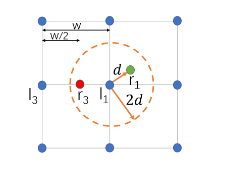
\includegraphics[width=0.7\linewidth]{img/Pasted image 20250331211545.png}
				
				\begin{itemize}
					\item To estimate the quality of joining $r_1$, we first find its nearest neighbor in $L$, which we’ll call $l_1$.
					\item Compute the distance: $d = f(l_1, r_1)$.
					\item Draw a ball of radius $2d$ centered at $l_1$.
					\begin{itemize}
						\item If no other $L$ records fall in the ball $\rightarrow$ high confidence.
					\end{itemize}
					\item In this case, the 2$d$-ball contains only $l_1$:
					$$
					\text{precision}(l_1, r_1) = \frac{1}{1} = 1
					$$
					\item \textbf{High confidence join}.
				\end{itemize}

			\end{beamercolorbox}
		\end{column}
	\end{columns}
\end{frame}
	


\begin{frame}{Theoretical foundation: When $L$ is incomplete}
	\begin{columns}
		\begin{column}{0.53\textwidth}
			\textbf{Problem:} When $L$ is incomplete (i.e., some records are missing):
			\begin{itemize}
				\item Missing records in $L$ result in \textbf{missing stars} in the grid.
				\item A record $r$ may join to the wrong $l$, causing \textbf{false positives} and reducing \textbf{precision}.
				\item Example: If $r_2$ should match with $l_2$ (but $l_2$ is missing), it might instead match $l_1$ using $d = f(r_2, l_1)$.
			\end{itemize}
			

			\textbf{Note:}
			\begin{itemize}
				\item Even if some records in $L$ are missing, \textbf{safe decisions} can still be made.
			\end{itemize}
			

			\textbf{Precision estimation:}
			\begin{itemize}
				\item $r_2$ should match $l_2$ (missing), so $l_1$ becomes the fallback.
				\item The 2$d'$-ball around $l_1$ contains \textbf{5 records}.
				\item Precision:
				$$
				\text{precision}(l_1, r_2) = \frac{1}{5}
				$$
				\item $\Rightarrow$ \textbf{Low confidence join}
			\end{itemize}
		\end{column}
		
		\begin{column}{0.43\textwidth}
			\begin{beamercolorbox}[rounded=true, shadow=true, leftskip=1em, rightskip=1em]{example}		
				\centering
				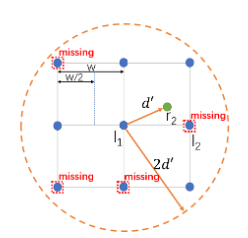
\includegraphics[width=0.7\linewidth]{img/Pasted image 20250331211607.png}
			
				\begin{itemize}
					\item $r_2$ should join with $l_2$, but $l_2$ is \textbf{missing}
					\item $l_1$ becomes the closest available record
					\item Compute distance $d' = f(l_1, r_2)$
					\item Draw a 2$d'$-ball around $l_1$
					\begin{itemize}
						\item If the ball includes many other $L$ records $\rightarrow$ $d'$ is too \textbf{lax}
						\item Join becomes unreliable
					\end{itemize}
				\end{itemize}
				
			\end{beamercolorbox}
		\end{column}
	\end{columns}
\end{frame}
	

\begin{frame}{Theoretical foundation: Estimating Precision and Recall for a configuration}
	
	\tiny	
	
	A configuration $C = \langle f, \theta \rangle$ includes:
	\begin{itemize}
		\item A join function $f$
		\item A threshold $\theta$
	\end{itemize}
	
	\textbf{1. Local precision for a join}
	
	\begin{beamercolorbox}[rounded=true, shadow=true, leftskip=1em, rightskip=1em]{definition}		
		$$
		\text{precision}(r, C) =
		\frac{1}{
			|\{ l' \in L \mid f(l, l') \leq 2f(l, r) \}|
		}
		$$
	\end{beamercolorbox}
	\begin{itemize}
		\item $J_C(r) = l$: join match for $r \in R$
		\item Denominator = number of plausible alternatives
	\end{itemize}
	
	\textbf{2. Expected true positives}
	\begin{beamercolorbox}[rounded=true, shadow=true, leftskip=1em, rightskip=1em]{definition}		
	$$
	TP(C) = \sum_{r \in R, J_C(r) \neq \emptyset} \text{precision}(r, C)
	$$
	\end{beamercolorbox}
	
	\textbf{3. Expected false positives}
	\begin{beamercolorbox}[rounded=true, shadow=true, leftskip=1em, rightskip=1em]{definition}		
	$$
	FP(C) = \sum_{r \in R, J_C(r) \neq \emptyset} \left(1 - \text{precision}(r, C)\right)
	$$
	\end{beamercolorbox}
	
	\textbf{4. Overall Precision and Recall}
	\begin{beamercolorbox}[rounded=true, shadow=true, leftskip=1em, rightskip=1em]{definition}		
	$$
	\text{precision}(C) = \frac{TP(C)}{TP(C) + FP(C)} \quad\quad
	\text{recall}(C) = TP(C)
	$$
	\end{beamercolorbox}
	
	\textit{Note:} Recall is estimated absolutely since ground truth is unavailable.
\end{frame}


\begin{frame}{Understanding TP and FP contributions}
	
	\textbf{True Positives (TP) and False Positives (FP)} are calculated from the estimated precision of each join:
	
	\vspace{0.5em}
	\begin{itemize}
		\item If a configuration joins a record $r$ with high estimated precision $\rightarrow$ contributes more to TP
		\item If a join has low estimated precision $\rightarrow$ contributes more to FP
	\end{itemize}
	
	\vspace{0.5em}
	\textbf{Formula Review:}
	\begin{align*}
		TP(C) &= \sum_{r \in R, J_C(r) \neq \emptyset} \text{precision}(r, C) \\
		FP(C) &= \sum_{r \in R, J_C(r) \neq \emptyset} \left(1 - \text{precision}(r, C)\right)
	\end{align*}
	
	\vspace{0.5em}
	\textbf{Implication:}
	\begin{itemize}
		\item Adding a configuration to $U$ increases recall (more joins)
		\item But can hurt precision if added joins are unreliable
		\item Greedy selection prefers configurations that give more TP per unit FP
	\end{itemize}
\end{frame}



	
\begin{frame}{Example: Precision and Recall estimation}
	
	\begin{beamercolorbox}[rounded=true, shadow=true, leftskip=1em, rightskip=1em]{example}		
	
		\textbf{Setup:} Assume 3 records in $R$, joined to $L$ using configuration $C = \langle f, \theta \rangle$.
		
		\vspace{0.5em}
		\textbf{Join Results:}
		\begin{itemize}
			\item $J_C(r_1) = l_1$, $f(l_1, r_1) = 0.1$, 5 plausible matches $\Rightarrow \text{precision}(r_1, C) = \frac{1}{5} = 0.20$
			\item $J_C(r_2) = l_2$, $f(l_2, r_2) = 0.05$, 2 plausible matches $\Rightarrow \text{precision}(r_2, C) = \frac{1}{2} = 0.50$
			\item $J_C(r_3) = l_3$, $f(l_3, r_3) = 0.2$, 4 plausible matches $\Rightarrow \text{precision}(r_3, C) = \frac{1}{4} = 0.25$
		\end{itemize}
		
		\vspace{0.5em}
		\textbf{Estimated TP and FP:}
		\begin{align*}
			TP(C) &= 0.20 + 0.50 + 0.25 = 0.95 \\
			FP(C) &= (1 - 0.20) + (1 - 0.50) + (1 - 0.25) = 2.05
		\end{align*}
	
		\vspace{0.5em}
		\textbf{Estimated Precision and Recall:}
		\begin{align*}
			\text{precision}(C) &= \frac{0.95}{0.95 + 2.05} = \frac{0.95}{3.00} \approx \textbf{0.317} \\\\
			\text{recall}(C) &= TP(C) = \textbf{0.95}
		\end{align*}
		
		\vspace{0.5em}
		\textit{Note:} This example assumes no ground truth; hence recall is based on expected TP count.
		
	\end{beamercolorbox}
	
\end{frame}


\begin{frame}{Theoretical foundation: Precision and Recall for a set of configurations}
	Let $U = \{C_1, C_2, \dots, C_K\}$ be a set of configurations.
	
	\vspace{0.5em}
	\textbf{Case 1: No Conflicts in $U$}
	\begin{itemize}
		\item Each record $r \in R$ is matched by at most one configuration:
		$$
		\forall r \in R, \quad |J_U(r)| \leq 1
		$$
		\item Then:
		$$
		TP(U) = \sum_{C \in U} TP(C), \quad
		FP(U) = \sum_{C \in U} FP(C)
		$$
	\end{itemize}
	
	\vspace{0.5em}
	\textbf{Case 2: Conflicting Assignments in $U$}
	\begin{itemize}
		\item Multiple configurations suggest different joins for the same $r$
		\item Resolve conflicts by:
		\begin{enumerate}
			\item Compare precision scores: $\text{precision}(r, C_i)$ vs. $\text{precision}(r, C_j)$
			\item Choose the match with higher precision
			\item Assign that join to $J_U(r)$
			\item Recompute $TP(U)$ and $FP(U)$
		\end{enumerate}
	\end{itemize}
	
	\vspace{0.5em}
	\textbf{Final Estimates:}
	$$
	\text{precision}(U) = \frac{TP(U)}{TP(U) + FP(U)} \qquad
	\text{recall}(U) = TP(U)
	$$
\end{frame}


\begin{frame}{Example: resolving conflicting joins from multiple configurations}
	
	\begin{beamercolorbox}[rounded=true, shadow=true, leftskip=1em, rightskip=1em]{example}		
	
		\textbf{Context:} Two configurations propose different joins for the same record $r \in R$ using different string similarity methods.
		
		\vspace{0.5em}
		\textbf{Configurations:}
		\begin{itemize}
			\item $C_1 = \langle f_1, \theta_1 \rangle$, where $f_1$ uses Jaccard distance over space-tokenized lowercase strings with equal weights.
			\item $C_2 = \langle f_2, \theta_2 \rangle$, where $f_2$ uses Cosine similarity over character trigrams with TF-IDF weighting.
		\end{itemize}
		
		\vspace{0.5em}
		\textbf{Join Proposals for $r$:}
		\begin{itemize}
			\item $C_1$: $J_{C_1}(r) = l_1$ with $\text{precision}(r, C_1) = \frac{1}{4} = 0.25$
			\item $C_2$: $J_{C_2}(r) = l_2$ with $\text{precision}(r, C_2) = \frac{1}{2} = 0.50$
		\end{itemize}
		
		\vspace{0.5em}
		\textbf{Conflict Resolution Strategy:}
		\begin{enumerate}
			\item Compare estimated precision:
			$$
			\text{precision}(r, C_1) = 0.25 < \text{precision}(r, C_2) = 0.50
			$$
			\item Assign $J_U(r) = l_2$ (higher-confidence match from $C_2$)
		\end{enumerate}
		
		\vspace{0.5em}
		\textbf{Effect:}
		\begin{itemize}
			\item $TP(U)$ and $FP(U)$ incorporate only the winning match.
			\item Competing matches are discarded.
		\end{itemize}
	
	\end{beamercolorbox}

\end{frame}


\begin{frame}{Auto-FuzzyJoin Algorithm: single column case}
	\begin{columns}
		\begin{column}{0.55\textwidth}
			\textbf Recall-Maximizing Fuzzy Join (RM-FJ) is \textbf{NP-hard}. Use a \textbf{greedy approximation algorithm} called \texttt{AutoFJ}.
			
			\vspace{0.5em}
			\textbf{Objective:}
			\begin{itemize}
				\item Maximize recall $TP(U)$ subject to maintaining $\text{precision}(U) \geq \tau$
			\end{itemize}
			
			\textbf{Greedy Strategy:}
			\begin{itemize}
				\item Select configurations that:
				\begin{itemize}
					\item Increase true positives (recall)
					\item Minimize false positives (preserve precision)
				\end{itemize}
				\item Guided by the \textbf{Profit Metric}:
				$$
				\text{profit}(U) = \frac{TP(U)}{FP(U)}
				$$
			\end{itemize}
			
			\textbf{Blocking Heuristic:}
			\tiny
			\begin{itemize}
				\item To reduce the number of comparisons, apply \textbf{3-gram blocking}.
				\item Each string is decomposed into overlapping sequences of 3 characters (3-grams).
				\item Only record pairs that share at least one common 3-gram are considered for joining.
				\item This blocks out obviously dissimilar pairs and speeds up computation.
				\item Applied to both $L$–$L$ and $L$–$R$ candidate pairs:
				$$
				LL, LR \leftarrow \text{generate candidate pairs using 3-gram overlap}
				$$
			\end{itemize}

		\end{column}
		
		\begin{column}{0.45\textwidth}
			\centering
			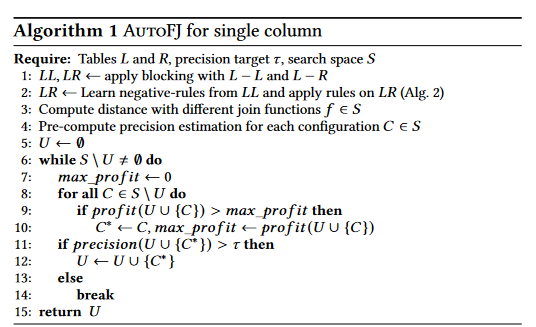
\includegraphics[width=\linewidth]{img/autofj-algorithm.png}
		\end{column}
	\end{columns}
\end{frame}

\begin{frame}{Problem formulation and complexity}
	
	\textbf{Goal:} Identify a set of join configurations $U \subseteq \mathcal{S}$ such that:
	\begin{itemize}
		\item Maximizes recall: $TP(U)$
		\item Satisfies precision constraint: $\text{precision}(U) \geq \tau$
	\end{itemize}
	
	\vspace{1em}
	\textbf{Formal problem definition: Recall-maximizing fuzzy join (RM-FJ)} \\
		
	\begin{beamercolorbox}[rounded=true, shadow=true, leftskip=1em, rightskip=1em]{definition}
		Given reference table $L$, query table $R$, and configuration space $\mathcal{S}$, find a subset $U \subseteq \mathcal{S}$ to:
		$$
		\max_{U \subseteq \mathcal{S}} TP(U) \quad \text{subject to} \quad \text{precision}(U) \geq \tau
		$$
	\end{beamercolorbox}
	
	\vspace{1em}
	\textbf{Computational Complexity:}
	\begin{itemize}
		\item The RM-FJ problem is shown to be \textbf{NP-hard}.
		\item Exact search over all subsets of $\mathcal{S}$ is computationally infeasible.
		\item Justifies use of \textbf{greedy approximation} (AutoFJ).
	\end{itemize}
	
\end{frame}

\begin{frame}{Blocking for efficient candidate generation}
	
	\textbf{Motivation:}
	\begin{itemize}
		\item Naively comparing every $r \in R$ with every $l \in L$ is computationally expensive.
		\item We use a \textbf{blocking} technique to generate a smaller candidate set for similarity evaluation.
	\end{itemize}
	
	\vspace{0.5em}
	\textbf{Technique: 3-Gram Blocking}
	\begin{itemize}
		\item Each string is decomposed into overlapping substrings of 3 characters (3-grams).
		\item Only consider $(r, l)$ pairs that share at least one common 3-gram.
		\item Applied on both $L$–$L$ (for negative rule learning) and $L$–$R$ (for actual join candidates).
	\end{itemize}
	
	\vspace{0.5em}
	\textbf{Impact:}
	\begin{itemize}
		\item Reduces the number of unnecessary comparisons.
		\item Increases efficiency without significant recall loss.
	\end{itemize}
	
\end{frame}



\begin{frame}{1. 3-Gram blocking using TF-IDF}
	

	\begin{beamercolorbox}[rounded=true, shadow=true, leftskip=1em, rightskip=1em]{code}
		\texttt{LL, LR $\leftarrow$ apply 3-gram blocking on $L–L$ and $L–R$}
	\end{beamercolorbox}
	
	
	\vspace{0.5em}
	

	\begin{beamercolorbox}[rounded=true, shadow=true, leftskip=1em, rightskip=1em]{example}
		\textbf{Reference Table $L$:}
		\begin{tabular}{ll}
			$l_1$ & \texttt{"john smith"} \\
			$l_2$ & \texttt{"jane smythe"} \\
			$l_3$ & \texttt{"alice johnson"}
		\end{tabular}
		
		\vspace{0.5em}
		\textbf{Query Record $r_1$:} \texttt{"jon smyth"}
		
		\vspace{0.5em}
		\textbf{Step 1: Preprocessing (P)}
		\begin{itemize}
			\item Lowercasing (already lowercase)
			\item Add padding for 3-grams: e.g., \texttt{"john smith"} $\rightarrow$ \texttt{"\#\#john\#smith\#\#"}
		\end{itemize}
		
		\vspace{0.5em}
		\textbf{Step 2: Tokenization (T)}
		\begin{itemize}
			\item $r_1$: \texttt{\#\#j, \#jo, jon, on\# , n\#s, \#sm, smy, myt, yth, th\#, h\#\#}
			\item $l_1$, $l_2$: similar 3-gram sequences
		\end{itemize}
		
		\vspace{0.5em}
		\textbf{Step 3: Token Weighting (W)}
		\begin{itemize}
			\item Use TF-IDF to emphasize rare, meaningful trigrams (e.g., \texttt{smy}, \texttt{yth})
			\item $r_1$–$l_2$: \textbf{High score(rare overlapping trigrams)}, $r_1$–$l_1$: Medium (more common overlap), $r_1$–$l_3$: Zero (no shared trigrams)
		\end{itemize}
		
		\vspace{0.5em}
		\textbf{Blocking Result:}
		\begin{itemize}
			\item Only compare $r_1$ with $l_1$, $l_2$ $\rightarrow$ prune $l_3$
		\end{itemize}
	\end{beamercolorbox}
	
	
\end{frame}


\begin{frame}{2. Optimization - filtering with negative rules}
	

	\begin{beamercolorbox}[rounded=true, shadow=true, leftskip=1em, rightskip=1em]{code}
		\texttt{LR $\leftarrow$ Learn negative-rules from \textit{LL} and apply rules on \textit{LR} (Alg. 2)}
	\end{beamercolorbox}

	\vspace{0.5em}

	\begin{beamercolorbox}[rounded=true, shadow=true, leftskip=1em, rightskip=1em]{example}
		\textit{\small Assumption: Although 3-gram blocking may have pruned $l_3$, we assume here it was retained due to weak overlap, allowing us to illustrate negative-rule filtering.}
		
		\vspace{1em}
		\textbf{Goal:} Use \textbf{obvious non-matches} in $L$–$L$ to learn rules that help \textbf{filter unlikely $L$–$R$ pairs} before costly distance computations.
		
		\vspace{0.5em}
		\textbf{Step 1: Generate $LL$ — Self-Join on $L$ using 3-gram blocking}
		
		\begin{tabular}{llll}
			\textbf{Pair} & \textbf{Shared 3-grams} & \textbf{Interpretation} \\
			\hline
			$l_1$ vs $l_2$ & \texttt{sm, smy, th}  & Possibly similar \\
			$l_1$ vs $l_3$ & \texttt{jo, on}       & Clearly different \\
			$l_2$ vs $l_3$ & Weak overlap          & Probably different \\
		\end{tabular}
		
		\vspace{0.5em}
		\textbf{Learn Negative Rule:} \\
		\textit{"If 3-gram overlap $\leq 2$, treat as a non-match."}
		
		\vspace{0.5em}
		\textbf{Step 2: Apply Rule on $LR$ Candidate Pairs}
		\begin{tabular}{lllll}
			\textbf{Pair} & \textbf{Overlap} & \textbf{Apply Rule?} & \textbf{Keep?} \\
			\hline
			$r_1$, $l_1$  & $\sim 4$  & No  & Yes \\
			$r_1$, $l_2$  & $\sim 5$  & No  & Yes \\
			$r_1$, $l_3$  & $\sim 1$  & Yes & No  \\
		\end{tabular}
		
		\vspace{0.5em}
		\textbf{Effect:} \textit{Filter out clearly irrelevant pairs early — no need to compute Jaccard or Edit Distance!}
	\end{beamercolorbox}
\end{frame}


\begin{frame}{3. Compute distances - apply join functions}
	
	\begin{beamercolorbox}[rounded=true, shadow=true, leftskip=1em, rightskip=1em]{code}
	\texttt{Compute distance with different join functions $f \in \mathcal{S}$}\\
	\texttt{Pre-compute precision estimation for each configuration $C \in \mathcal{S}$}
	\end{beamercolorbox}
	
	\vspace{0.5em}
	Once candidate pairs are identified (via blocking and optional negative rules), we compute the actual similarity using multiple join functions $f \in \mathcal{S}$.
	
	\vspace{0.5em}
	\textbf{Each join function is defined by:}
	\begin{itemize}
		\item Preprocessing (e.g., lowercasing, punctuation removal)
		\item Tokenization (e.g., char 3-grams, word tokens)
		\item Token weights (e.g., TF-IDF)
		\item Distance function (e.g., Jaccard, Cosine, Edit)
	\end{itemize}
	
	\vspace{0.5em}
	\begin{beamercolorbox}[rounded=true, shadow=true, leftskip=1em, rightskip=1em]{example}
		\textbf{Example Candidate Pairs (after blocking):}
		\begin{tabular}{ll}
			$r$ (query) & $l$ (reference) \\
			\hline
			\texttt{"jon smyth"} & \texttt{"john smith"} \\
			\texttt{"jon smyth"} & \texttt{"jane smythe"} \\
		\end{tabular}
		
		\vspace{0.5em}
		\textbf{Join Functions in $\mathcal{S}$:}
		\begin{tabular}{llll}
			\textbf{Function $f$} & \textbf{Tokenizer} & \textbf{Distance} & \textbf{Description} \\
			\hline
			$f_1$ & char 3-grams & Jaccard & Overlap in token sets \\
			$f_2$ & char 3-grams & Cosine (TF-IDF) & Weighted similarity \\
			$f_3$ & raw string   & Levenshtein & Edit distance \\
		\end{tabular}
		
		\vspace{0.5em}
		\textbf{Computed Scores:}
		\begin{tabular}{lccc}
			\textbf{Pair} & $f_1$ & $f_2$ & $f_3$ \\
			\hline
			\texttt{jon vs john} & 0.4 & 0.5 & 2 \\
			\texttt{jon vs jane} & 0.6 & 0.7 & 3 \\
		\end{tabular}
		
		\vspace{0.5em}
		\textit{Note: Distances may follow different scales — lower often means more similar.}
	\end{beamercolorbox}
\end{frame}




\begin{frame}{4. Start of greedy algorithm}
	
	\begin{beamercolorbox}[rounded=true, shadow=true, leftskip=1em, rightskip=1em]{code}
	\texttt{\textbf{Initialize:} $U \leftarrow \emptyset$}
	\end{beamercolorbox}
	
		
	\vspace{1em}
	$U$ will hold the \textbf{selected join configurations}:
	$$
	C = \langle f, \theta \rangle
	$$
	
	Each configuration includes:
	\begin{itemize}
		\item A join function $f \in \mathcal{F}$ (defined by $P$, $T$, $W$, $D$)
		\item A distance threshold $\theta$ (max allowed distance for a match)
	\end{itemize}
	
	\vspace{0.5em}
	\textbf{Goal:}
	\begin{itemize}
		\item Select a subset $U \subseteq \mathcal{S}$ from all candidate configurations
		\item Maximize recall: $TP(U)$
		\item Maintain precision: $\text{precision}(U) \geq \tau$
	\end{itemize}
	
	\vspace{0.5em}
	\begin{beamercolorbox}[rounded=true, shadow=true, leftskip=1em, rightskip=1em]{example}
		\textbf{Example: Precomputed configuration set $S$}
		\begin{tabular}{ll}
			\textbf{Config $C$} & \textbf{Description} \\
			\hline
			$C_1 = \langle f_1, 0.37 \rangle$ & Jaccard distance with $\theta = 0.37$ \\
			$C_2 = \langle f_2, 0.42 \rangle$ & Cosine distance with $\theta = 0.42$ \\
			$C_3 = \langle f_3, 2 \rangle$    & Edit distance with $\theta = 2$ \\
		\end{tabular}
		
		\vspace{0.5em}
		\textit{These $\theta$ values were selected based on prior precision–recall evaluation for each $f$.}
		
	\end{beamercolorbox}
	
\end{frame}


\begin{frame}{5. Main greedy loop}
	
	\begin{beamercolorbox}[rounded=true, shadow=true, leftskip=1em, rightskip=1em]{code}	
	\texttt{\textbf{Main Loop:} while } $S \setminus U \neq \emptyset$ \texttt{ do}
	\end{beamercolorbox}
	\vspace{0.5em}
	We continue as long as there are still unused configurations to consider.
	
	\vspace{0.5em}
	\textbf{Notation:}
	\begin{itemize}
		\item $S$: full set of candidate configurations, each $C = \langle f, \theta \rangle$
		\item $U$: set of selected configurations
		\item $S \setminus U$: unused configurations
	\end{itemize}
	
	\vspace{0.5em}
	\textbf{At each iteration:}
	\begin{enumerate}
		\item Evaluate each $C \in S \setminus U$
		\item Compute profit: how many true positives vs. false positives it contributes
		\item Select the best configuration $C^*$
		\item If $\text{precision}(U \cup \{C^*\}) \geq \tau$:
		\begin{itemize}
			\item[] \texttt{$U \leftarrow U \cup \{C^*\}$}
		\end{itemize}
	\end{enumerate}
	
	\vspace{0.5em}
	\begin{beamercolorbox}[rounded=true, shadow=true, leftskip=1em, rightskip=1em]{example}	
		\textbf{Example state:}
		\begin{itemize}
			\item $S = \{ \langle f_1, 0.37 \rangle, \langle f_2, 0.42 \rangle, \langle f_3, 2 \rangle \}$
			\item $U = \emptyset$
		\end{itemize}
		
		\textit{Loop continues while there are remaining candidates and precision can be preserved.}
	\end{beamercolorbox}
		
\end{frame}

\begin{frame}{6. Find most promising configuration (profit heuristic)}
	
	\begin{beamercolorbox}[rounded=true, shadow=true, leftskip=1em, rightskip=1em]{code}	
	\begin{itemize}
		\item[] \texttt{max\_profit ← 0}
		\item[] \texttt{for all } $C \in S \setminus U$ \texttt{ do}
		\begin{itemize}
			\item[] \texttt{if } $\text{profit}(U \cup \{C\}) > \texttt{max\_profit}$ \texttt{ then}
			\item[] \quad $C^* \leftarrow C$, $\texttt{max\_profit} \leftarrow \text{profit}(U \cup \{C\})$
		\end{itemize}
	\end{itemize}
	\end{beamercolorbox}
	
	\vspace{0.5em}
	\textbf{Profit Formula:}
	$$
	\text{profit}(U \cup \{C\}) = \frac{TP(U \cup \{C\})}{FP(U \cup \{C\})}
	$$
	
	\vspace{0.5em}
	\begin{beamercolorbox}[rounded=true, shadow=true, leftskip=1em, rightskip=1em]{example}		
	\textbf{Example:}
	\begin{tabular}{lccc}
		\textbf{Config $C$} & \textbf{TP} & \textbf{FP} & \textbf{Profit = TP / FP} \\
		\hline
		$C_1$ & 4 & 2 & 2.0 \\
		$C_2$ & 5 & 5 & 1.0 \\
		$C_3$ & 3 & 1 & \textbf{3.0} \\
	\end{tabular}
	
	\vspace{0.5em}
	After evaluation: $C^* = C_3$, $\texttt{max\_profit} = 3.0$
	\end{beamercolorbox}
	
	\vspace{0.5em}

	\textit{Heuristic: choose the configuration that gives the most recall “bang” per unit of precision “risk.”}

\end{frame}

\begin{frame}{7. Precision constraint check \& termination}
	
	\begin{beamercolorbox}[rounded=true, shadow=true, leftskip=1em, rightskip=1em]{code}	
	\texttt{\textbf{Check:} if } $\text{precision}(U \cup \{C^*\}) > \tau$ \texttt{ then}  
	\quad \texttt{$U \leftarrow U cup \{C^*\}$}
	\end{beamercolorbox}
	
	\vspace{0.5em}
	After selecting the best candidate $C^*$ (based on profit), we must verify that adding it to $U$ preserves minimum required precision $\tau$.
	
	\begin{itemize}
		\item If precision passes: add $C^*$ to $U$
		\item Else: break — no remaining configs will satisfy the constraint
	\end{itemize}
	
	\vspace{1em}
	\begin{beamercolorbox}[rounded=true, shadow=true, leftskip=1em, rightskip=1em]{example}		
	\textbf{Example 1 (Pass):}
	\begin{tabular}{lccccc}
		Config & TP & FP & Profit & Precision & $\tau$ \\
		\hline
		$C_3$ & 3 & 1 & 3.0 & \textbf{0.75} & 0.7 \\
	\end{tabular}
	
	\vspace{0.5em}
	$\Rightarrow$ Precision $>$ $\tau$ $\rightarrow$ Accept $\rightarrow$ $U \leftarrow \{C_3\}$
	
	\vspace{1em}
	\textbf{Example 2 (Fail \& Break):}
	\begin{tabular}{lccccc}
		Config & TP & FP & Profit & Precision & $\tau$ \\
		\hline
		$C_3$ & 3 & 1 & 3.0 & \textbf{0.75} & 0.8 \\
	\end{tabular}
	
	\vspace{0.5em}
	$\Rightarrow$ Precision $<$ $\tau$ $\rightarrow$ Reject $\rightarrow$ Stop Loop
	\end{beamercolorbox}

	\vspace{0.5em}

	
	\textit{Greedy termination: If best config can’t meet $\tau$, no others will.}
\end{frame}


\begin{frame}{8. Return final join plan}
	
	\begin{beamercolorbox}[rounded=true, shadow=true, leftskip=1em, rightskip=1em]{code}		
	\texttt{\textbf{Return:} U}
	\end{beamercolorbox}
		
	\vspace{0.5em}
	The greedy loop terminates when:
	\begin{itemize}
		\item $S \setminus U = \emptyset$ (all configs evaluated), or
		\item The best candidate fails the precision constraint
	\end{itemize}
	
	\vspace{0.5em}
	The algorithm returns $U$: a set of selected configurations:
	\begin{itemize}
		\item Each $C = \langle f, \theta \rangle$
		\item Maximizes recall while keeping $\text{precision}(U) \geq \tau$
	\end{itemize}
	
	\vspace{0.5em}
	\textbf{Each configuration in $U$ defines:}
	\begin{itemize}
		\item A join function $f$ (e.g., Jaccard, Cosine, Edit Distance)
		\item A threshold $\theta$ used to accept matches
	\end{itemize}
	
	\vspace{0.5em}
	\begin{beamercolorbox}[rounded=true, shadow=true, leftskip=1em, rightskip=1em]{example}		
	\textbf{Example Output:}
	\begin{itemize}
		\item $U = \{ \langle f_2 = \text{Cosine}, \theta = 0.5 \rangle,\ \langle f_3 = \text{Edit}, \theta = 2 \rangle \}$
	\end{itemize}
	\end{beamercolorbox}
		
	\textit{These are used to perform the final fuzzy similarity join.}
\end{frame}


\begin{frame}{Example: Selecting the best match}
	
	\begin{beamercolorbox}[rounded=true, shadow=true, leftskip=1em, rightskip=1em]{example}		
		\textbf{1. Input Setup:}
		\begin{itemize}
			\item Query record: $r_1$ = \texttt{"jon smyth"}
			\item Reference table: $L = \{\texttt{"john smith"},\ \texttt{"jane smythe"},\ \texttt{"alice johnson"}\}$
			\item After blocking: candidates for $r_1$ are $l_1$ and $l_2$
		\end{itemize}
		
		\vspace{0.5em}
		\textbf{2. Distance Results:}
		\begin{tabular}{lcccc}
			Join Function $f$ & $\theta$ & $f(r_1, l_1)$ & $f(r_1, l_2)$ & Matches? \\
			\hline
			Jaccard (3-grams) & 0.4 & 0.5 & 0.3 & $l_2$ only \\
			Cosine (TF-IDF)   & 0.5 & 0.6 & 0.4 & $l_2$ only \\
			Edit Distance     & 2.0 & 2 & 3 & $l_1$ only \\
		\end{tabular}
		
		\vspace{0.5em}
		\textbf{3. Final Configuration Set $U$:}
		\begin{itemize}
			\item $U = \{ \langle f_2 = \text{Cosine},\ \theta = 0.5 \rangle,\ \langle f_3 = \text{Edit},\ \theta = 2 \rangle \}$
			\item Under Cosine: $r_1 \mapsto l_2$
			\item Under Edit Distance: $r_1 \mapsto l_1$
		\end{itemize}
		
		\vspace{0.5em}
		\textbf{4. Conflict Resolution: Local Precision}
		
		\vspace{0.25em}
		$\text{precision}(r, C) = \frac{1}{\left| \{ l' \in L \mid f(l, l') \leq 2f(l, r) \} \right|}$
		
		\begin{tabular}{lcccc}
			Config $C$ & Match & $f(l, r)$ & $2d$-ball size & Precision \\
			\hline
			$C_2$ (Cosine) & $l_2$ & 0.4 & 5 & 1/5 = 0.2 \\
			$C_3$ (Edit)   & $l_1$ & 2 & 2 & \textbf{1/2 = 0.5} \\
		\end{tabular}
		
		\vspace{0.5em}
		\textbf{Result:} \textit{"jon smyth" is matched to "john smith" (Edit Distance), since it has higher estimated precision ($0.5 > 0.2$).}
	\end{beamercolorbox}
			
\end{frame}



\end{document}
